\documentclass[12pt,letterpaper]{article}
\usepackage[utf8]{inputenc}
\usepackage[margin=1in]{geometry}
\usepackage{graphicx}
\usepackage{titling}
\usepackage{amsmath}
\usepackage{amsfonts}
\usepackage{amssymb}
\renewcommand{\theenumiv}{\arabic{enumiv}}
\setlength{\droptitle}{-5em}
\author{Maurice Diesendruck}
\title{StatMod2 - Gibbs - Exercises 4}
\usepackage{Sweave}
\begin{document}
\input{statmod-gibbs-concordance}
\maketitle


\section{Model}
\begin{align*}
  \pmb{y} &\sim\ N(X\pmb{\beta}, \sigma^2\pmb{I_n})
		\text{ for i.i.d. } y_1, \cdots, y_n\\
	\pmb{\beta}|\tau^2 &\sim\ N(\pmb{0}, \tau^2\pmb{I_p})
		\text{ for i.i.d. } \beta_1, \cdots, \beta_p\\
	\sigma^2 &\sim\ IG(a/2, b/2) \equiv
		\Big(\frac{1}{\sigma^2} \Big) \sim\ Ga(a/2, b/2) \hspace{2mm}\dagger\\
	\tau^2 &\sim\ IG(c/2, d/2)\equiv
		\Big(\frac{1}{\sigma^2} \Big) \sim\ Ga(a/2, b/2) \hspace{2mm}\dagger\\
	\dagger &\text{ For notational convenience, the following distributions
		use } Ga(a, b){.}\\
		& \text{ In R, } a \text{ and } b \text{ are initialized as 1/2.}
\end{align*}

\section{Joint Posterior}
Let $\pmb{\theta} = (\pmb{\beta}, \sigma^2, \tau^2)$.
\begin{align*}
	P(\pmb{\theta}|y) &\propto\ P(y|\pmb{\theta})P(\pmb{\theta})\\
	&= N(y|X\pmb{\beta},\sigma^2)
		N(\pmb{\beta}|\pmb{0}, \tau^2\pmb{I_p})
		Ga(\dfrac{1}{\sigma^2}|a, b) Ga(\dfrac{1}{\tau^2}|c, d)\\
	&\propto\ \Big( \dfrac{1}{\sigma^2} \Big) ^{n/2} 
		exp \Big( -\frac{1}{2} \Big( \dfrac{(\pmb{y}-X\pmb{\beta})'
			(\pmb{y}-X\pmb{\beta})} {\sigma^2} \Big) \Big)\\
		&\hspace{10mm} \text{x } \Big( \dfrac{1}{\tau^2} \Big) ^{p/2}
			exp \Big( -\frac{1}{2} \dfrac{\pmb{\beta}'\pmb{\beta}}{\tau^2}
			\Big)\Big)\\
		& \hspace{10mm} \text{x } \Big( \dfrac{1}{\sigma^2} \Big) 
			^{a-1} exp^{-b \Big( \dfrac{1}{\sigma^2} \Big)}\\
		& \hspace{10mm} \text{x } \Big( \dfrac{1}{\tau^2} \Big) 
			^{c-1} exp^{-d \Big( \dfrac{1}{\tau^2} \Big)}\\
\end{align*}

\section{Full Conditionals}
\begin{align*}
P(\pmb{\beta}|\pmb{y}, \sigma^2, \tau^2) &\propto\
	exp \Big( -\frac{1}{2} \Big( \dfrac{(\pmb{y}-X\pmb{\beta})'
			(\pmb{y}-X\pmb{\beta})} {\sigma^2} + 
			\dfrac{\pmb{\beta}'\pmb{\beta}}{\tau^2}
			\Big) \Big)\\
	&= exp \Big( -\frac{1}{2} \Big( 
		\dfrac{\pmb{y}'\pmb{y}}{\sigma^2}
		- \dfrac{\pmb{y}'X\pmb{\beta}}{\sigma^2}
		- \dfrac{\pmb{\beta}'X'\pmb{y}}{\sigma^2}
		+ \beta' ( \frac{X'X}{\sigma^2} + \frac{I_p}{\tau^2} ) \beta 
		\Big) \Big)\\
	&\sim\ N \Bigg( \Big( \frac{X'X}{\sigma^2} + \frac{I_p}{\tau^2} \Big) ^{-1}
		\frac{X'Y}{\sigma^2} , 
		\Big( \frac{X'X}{\sigma^2} + \frac{I_p}{\tau^2} \Big) ^{-1}
		\Bigg)\\
\vspace{10mm}\\
P(\sigma^2|\pmb{y},\pmb{\beta},\tau^2) &\propto\
	\Big( \dfrac{1}{\sigma^2} \Big) ^{n/2}
	exp \Big( -\frac{1}{2} \Big( \dfrac{(\pmb{y}-X\pmb{\beta})'
			(\pmb{y}-X\pmb{\beta})} {\sigma^2} \Big) \Big)\\
	& \hspace{10mm} \text{x } \Big( \dfrac{1}{\sigma^2} \Big) 
			^{a-1} exp^{-b \Big( \dfrac{1}{\sigma^2} \Big)}\\
	&= \Big( \dfrac{1}{\sigma^2} \Big) ^{n/2 + a -1}
		exp \Big( - \Big( \dfrac{(\pmb{y}-X\pmb{\beta})'
			(\pmb{y}-X\pmb{\beta})} {2} + b \Big)
			\Big( \frac{1}{\sigma^2} \Big) \Big)\\
	&\sim\ Ga \Big( n/2+a, \Big( \dfrac{(\pmb{y}-X\pmb{\beta})'
			(\pmb{y}-X\pmb{\beta})} {2} + b \Big) \Big)\\
\vspace{10mm}\\
P(\tau^2|\pmb{y},\pmb{\beta},\sigma^2) &\propto\
	\Big( \dfrac{1}{\tau^2} \Big) ^{p/2}
	exp \Big( -\frac{1}{2} \Big( \dfrac{\pmb{\beta}'\pmb{\beta}}{\tau^2}
			\Big) \Big)\\
	& \hspace{10mm} \text{x } \Big( \dfrac{1}{\tau^2} \Big) 
			^{c-1} exp^{-d \Big( \dfrac{1}{\tau^2} \Big)}\\
	&= \Big( \dfrac{1}{\tau^2} \Big) ^{p/2 + c -1}
		exp \Big( - \Big( \dfrac{\pmb{\beta}'\pmb{\beta}}{2} + d \Big)
			\Big( \frac{1}{\tau^2} \Big) \Big)\\
	&\sim\ Ga \Big( p/2+c, \Big( \dfrac{\pmb{\beta}'\pmb{\beta}}{2}
		 + d \Big) \Big)\\
\end{align*}

\section{Results}

These are the means of $\beta_1,\cdots,\beta_p$. Each also mixed appropriately.

\begin{Schunk}
\begin{Soutput}
 [1]   -2.051309 -221.537769  510.610845  310.677515 -180.066386   -7.965675
 [7] -159.422452  111.922047  507.486380   77.530884
\end{Soutput}
\end{Schunk}

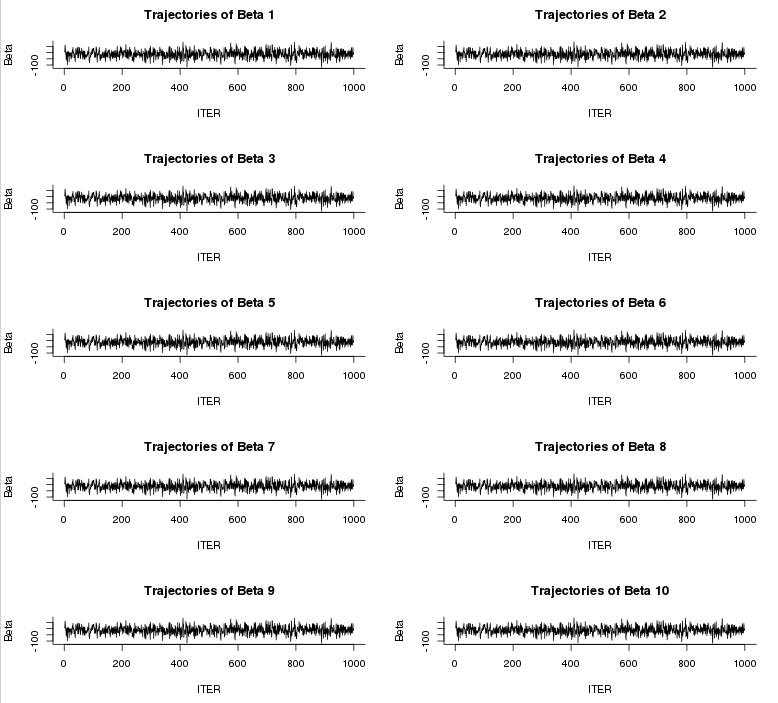
\includegraphics{betas.png}

\includegraphics{statmod-gibbs-002}


\end{document}
